\documentclass[aspectratio=169]{beamer}
\usetheme{Madrid}
\usecolortheme{default}
\usepackage[utf8]{inputenc}
\usepackage[T5]{fontenc}
\usepackage{graphicx}
\usepackage{hyperref}
\usepackage{booktabs}
\usepackage{amsmath}
\usepackage{listings}
\usepackage{color}

\definecolor{codegreen}{rgb}{0,0.6,0}
\definecolor{codegray}{rgb}{0.5,0.5,0.5}
\definecolor{codepurple}{rgb}{0.58,0,0.82}
\definecolor{backcolour}{rgb}{0.95,0.95,0.92}

\lstdefinestyle{mystyle}{
    backgroundcolor=\color{backcolour},   
    commentstyle=\color{codegreen},
    keywordstyle=\color{magenta},
    numberstyle=\tiny\color{codegray},
    stringstyle=\color{codepurple},
    basicstyle=\ttfamily\scriptsize,
    breakatwhitespace=false,         
    breaklines=true,                 
    captionpos=b,                    
    keepspaces=true,                 
    numbers=left,                    
    numbersep=5pt,                  
    showspaces=false,                
    showstringspaces=false,
    showtabs=false,                  
    tabsize=2
}
\lstset{style=mystyle}

\setbeamertemplate{caption}[numbered]
\renewcommand{\figurename}{Hình}
\renewcommand{\thefigure}{17.\arabic{figure}}

\title[Chương 17: Image Generation]{Học Sâu (Deep Learning) \\ \vspace{0.5cm} \Large Chương 17: Trí tuệ Nhân tạo Sinh ảnh (Image Generation)}
\author{Đại học Đông Á}
\date{\today}

\begin{document}

\begin{frame}
    \titlepage
\end{frame}

\begin{frame}{Nội dung chương}
    \tableofcontents
\end{frame}

\section{1. Không gian tiềm ẩn \& Text-to-Image}

\begin{frame}{Khái quát về Sinh ảnh (Image Generation)}
    \begin{columns}
        \column{0.5\textwidth}
        \begin{itemize}
            \item Ý tưởng cốt lõi của việc sinh ảnh là phát triển một \textbf{Không gian tiềm ẩn (Latent Space)} với số chiều thấp.
            \item Bất kỳ điểm nào trong không gian này đều có thể được một bộ \textbf{Generator/Decoder} ánh xạ thành một bức ảnh hợp lệ.
            \item AI không hề sao chép, nó Lấy mẫu (Sample) một tọa độ mới hoàn toàn và sinh ra bức ảnh chưa từng tồn tại.
        \end{itemize}
        
        \column{0.5\textwidth}
        \begin{figure}
            \centering
            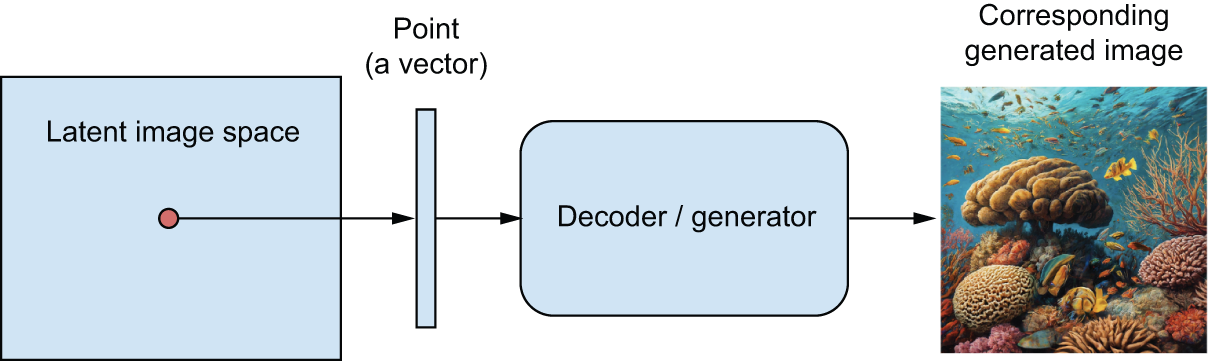
\includegraphics[width=\textwidth,height=0.6\textheight,keepaspectratio]{../../images/ch17/image_gen.d02c5d8f.png}
            \caption{Sử dụng Không gian tiềm ẩn để lấy mẫu ảnh mới}
        \end{figure}
    \end{columns}
\end{frame}

\begin{frame}{Mô hình Text-to-Image (Văn bản thành Hình ảnh)}
    \begin{columns}
        \column{0.5\textwidth}
        \begin{itemize}
            \item Bằng cách ánh xạ không gian văn bản (Text embedding) vào cùng không gian tiềm ẩn của hình ảnh (Image Latent Space).
            \item Ta có thể sinh ảnh dựa trên sự điều hướng của ngôn ngữ tự nhiên. VD: \textit{"Một con ngựa đạp xe trên mặt trăng"}.
            \item Dù AI chưa từng thấy bức ảnh nào như vậy, nó vẫn nội suy được từ các khái niệm rời rạc.
        \end{itemize}
        
        \column{0.5\textwidth}
        \begin{figure}
            \centering
            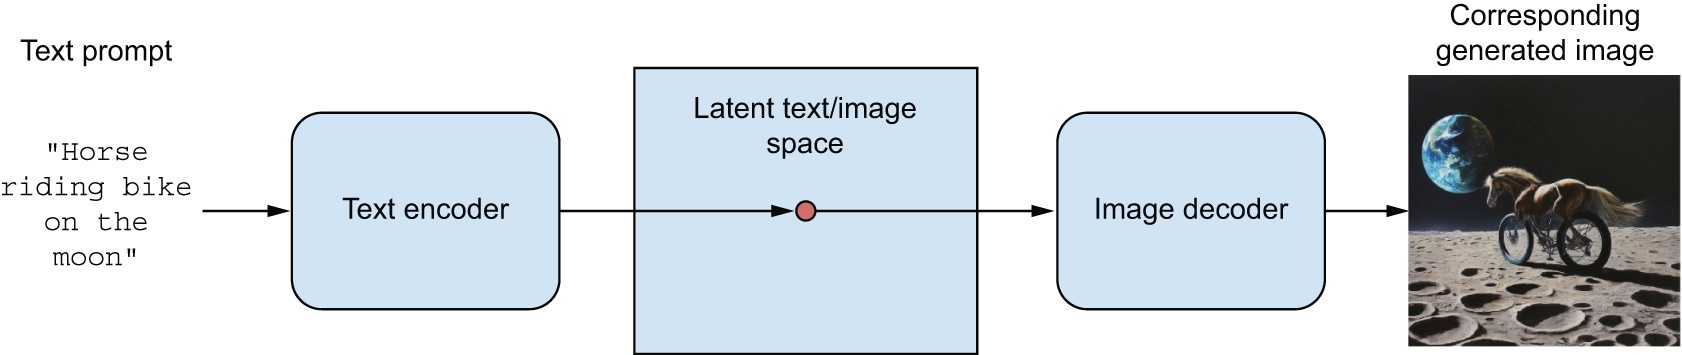
\includegraphics[width=\textwidth,height=0.6\textheight,keepaspectratio]{../../images/ch17/text-to-image.d51ae48c.png}
            \caption{Sinh ảnh bằng điều hướng Ngôn ngữ}
        \end{figure}
    \end{columns}
\end{frame}

\begin{frame}{Bộ dữ liệu kinh điển: Oxford Flowers}
    \begin{columns}
        \column{0.5\textwidth}
        \begin{itemize}
            \item Trong chương này, chúng ta sẽ thực hành huấn luyện AI sinh ảnh trên bộ dữ liệu \textbf{Oxford Flowers 102}.
            \item Nó bao gồm hàng ngàn bức ảnh hoa với đủ màu sắc, hình dáng, là "chuột bạch" lý tưởng cho các mô hình sinh ảnh như VAE hay Diffusion.
            \item Hình ảnh sẽ được resize về kích thước chuẩn $128 \times 128$ trong quá trình tiền xử lý.
        \end{itemize}
        
        \column{0.5\textwidth}
        \begin{figure}
            \centering
            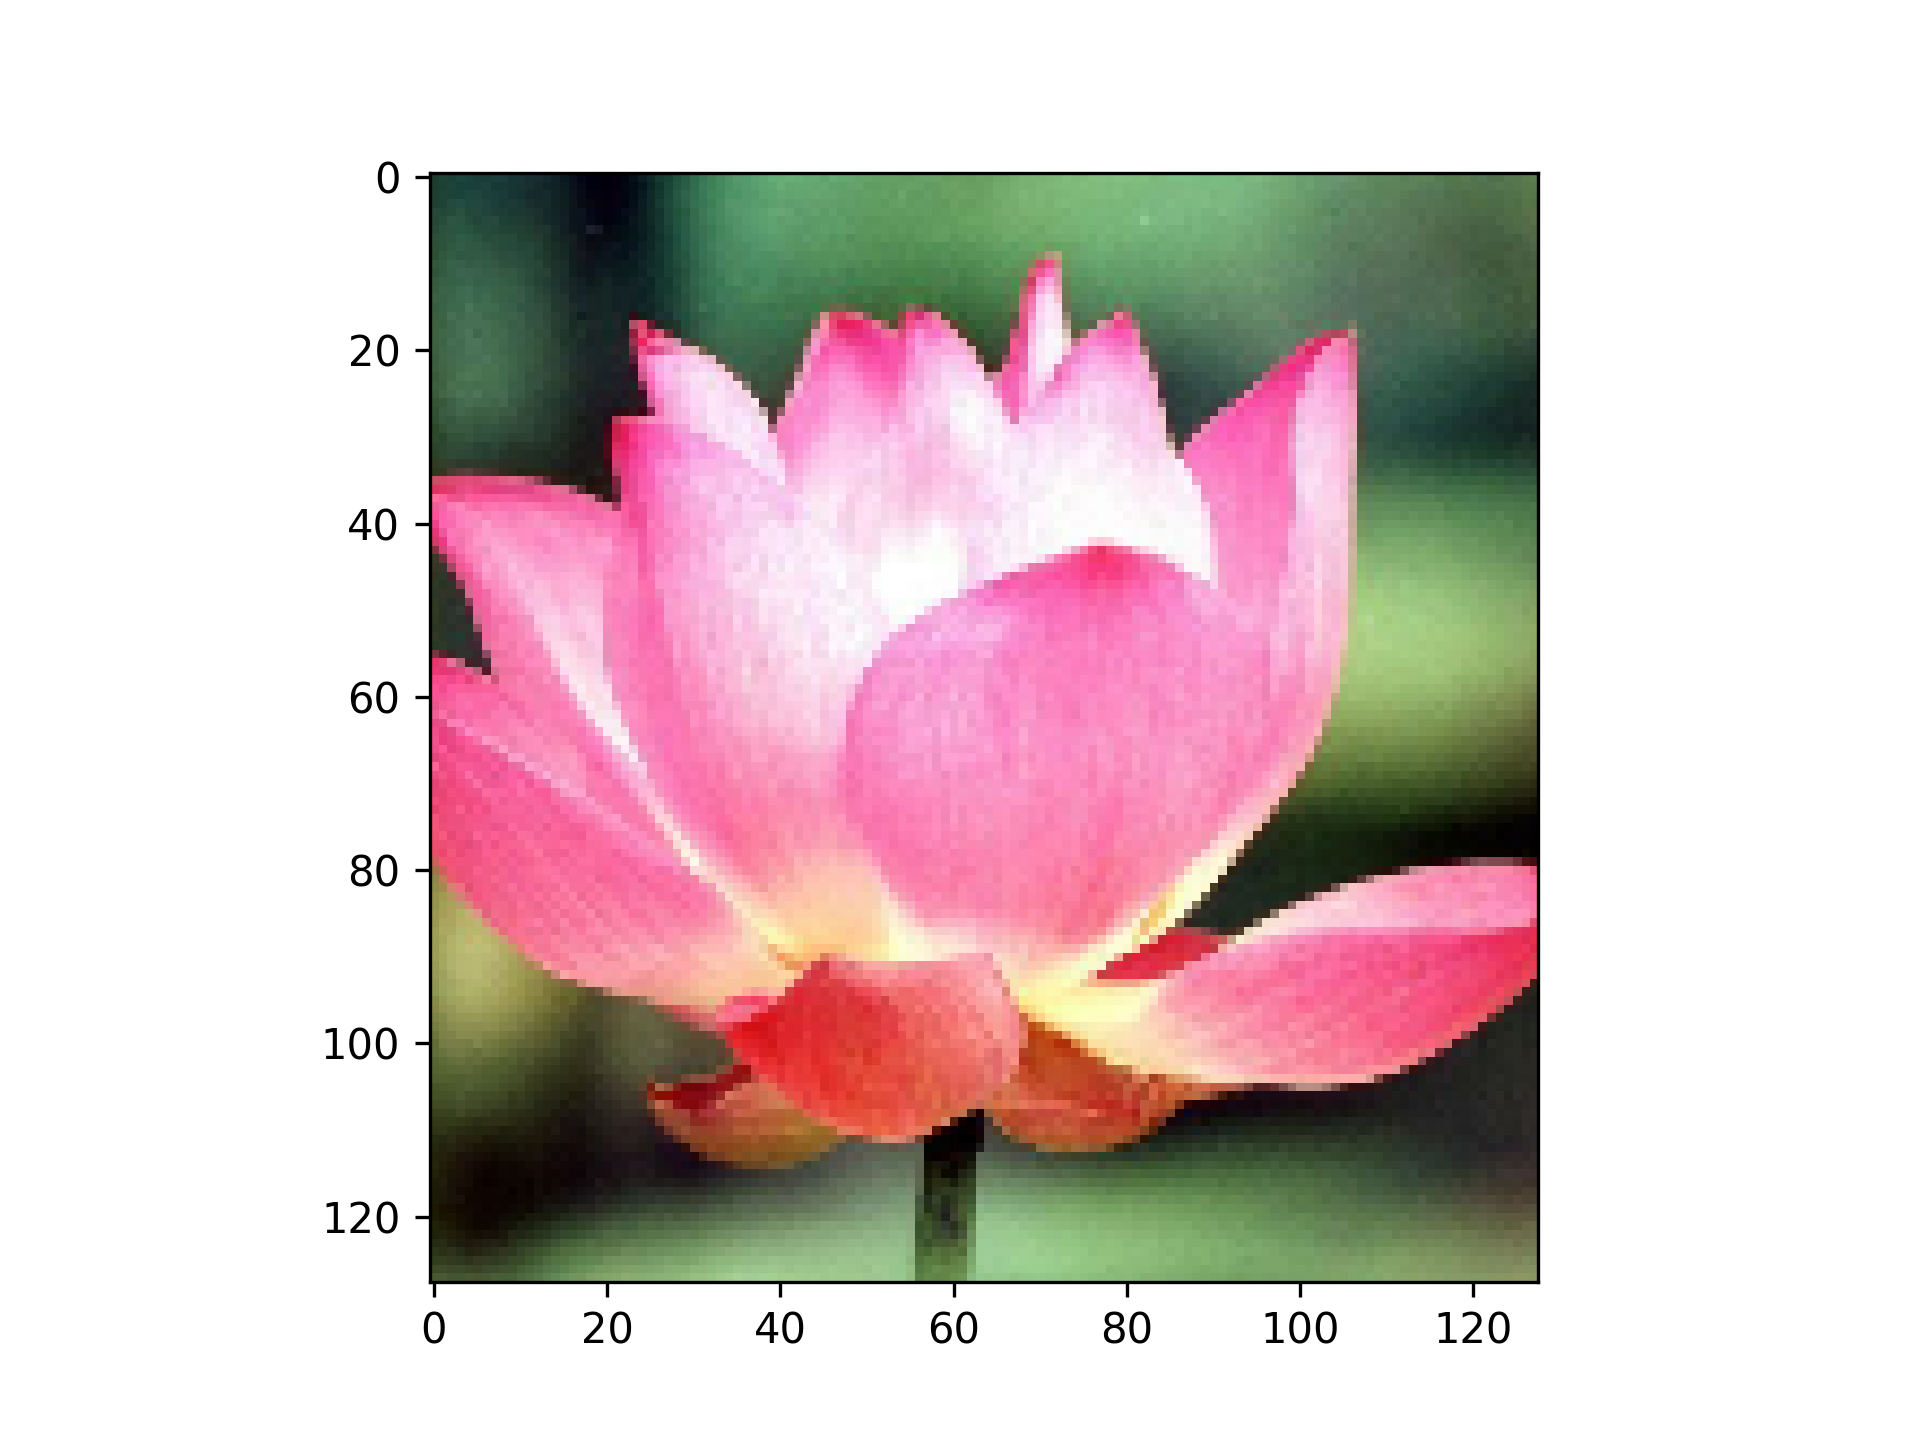
\includegraphics[width=\textwidth,height=0.6\textheight,keepaspectratio]{../../images/ch17/oxford_flower.215934bb.png}
            \caption{Một số mẫu từ bộ dữ liệu Oxford Flower}
        \end{figure}
    \end{columns}
\end{frame}

\section{2. Mạng Variational Autoencoders (VAEs)}

\begin{frame}{Giới hạn của Autoencoder truyền thống}
    \begin{columns}
        \column{0.5\textwidth}
        \begin{itemize}
            \item Mạng Autoencoder gồm 2 phần: Encoder nén ảnh thành mã (code) và Decoder giải nén mã về lại ảnh ban đầu.
            \item Tuy nhiên, Không gian tiềm ẩn (Latent space) của nó bị \textbf{đứt gãy}. Nếu lấy một điểm ngẫu nhiên ở giữa không gian, Decoder sẽ nhả ra một bức ảnh rác vô nghĩa.
        \end{itemize}
        
        \column{0.5\textwidth}
        \begin{figure}
            \centering
            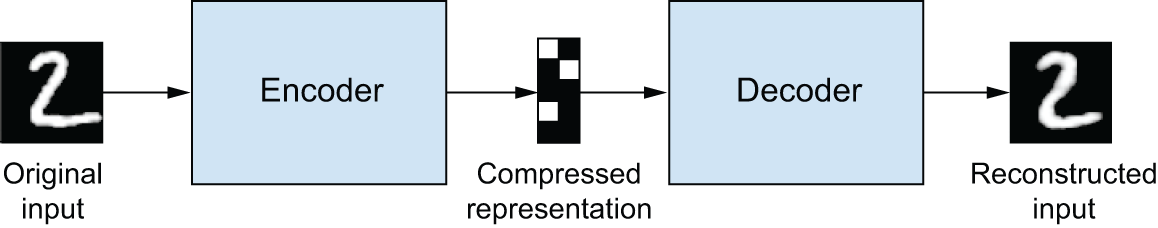
\includegraphics[width=\textwidth,height=0.6\textheight,keepaspectratio]{../../images/ch17/autoencoder.71a857ef.png}
            \caption{Autoencoder truyền thống}
        \end{figure}
    \end{columns}
\end{frame}

\begin{frame}{Sự đột phá của Variational Autoencoder (VAE)}
    \begin{columns}
        \column{0.5\textwidth}
        \begin{itemize}
            \item VAE (2013) không nén ảnh thành 1 điểm cứng nhắc. Nó nén ảnh thành một \textbf{Phân phối xác suất} (Phân phối chuẩn hình chuông).
            \item Thay vì xuất ra tọa độ $z$, Encoder xuất ra \textbf{Trung bình (Mean)} và \textbf{Phương sai (Variance)}.
            \item Không gian tiềm ẩn giờ đây liên tục và trơn tru. Bất kỳ điểm nào lấy mẫu (Sample) cũng sinh ra ảnh hợp lệ.
        \end{itemize}
        
        \column{0.5\textwidth}
        \begin{figure}
            \centering
            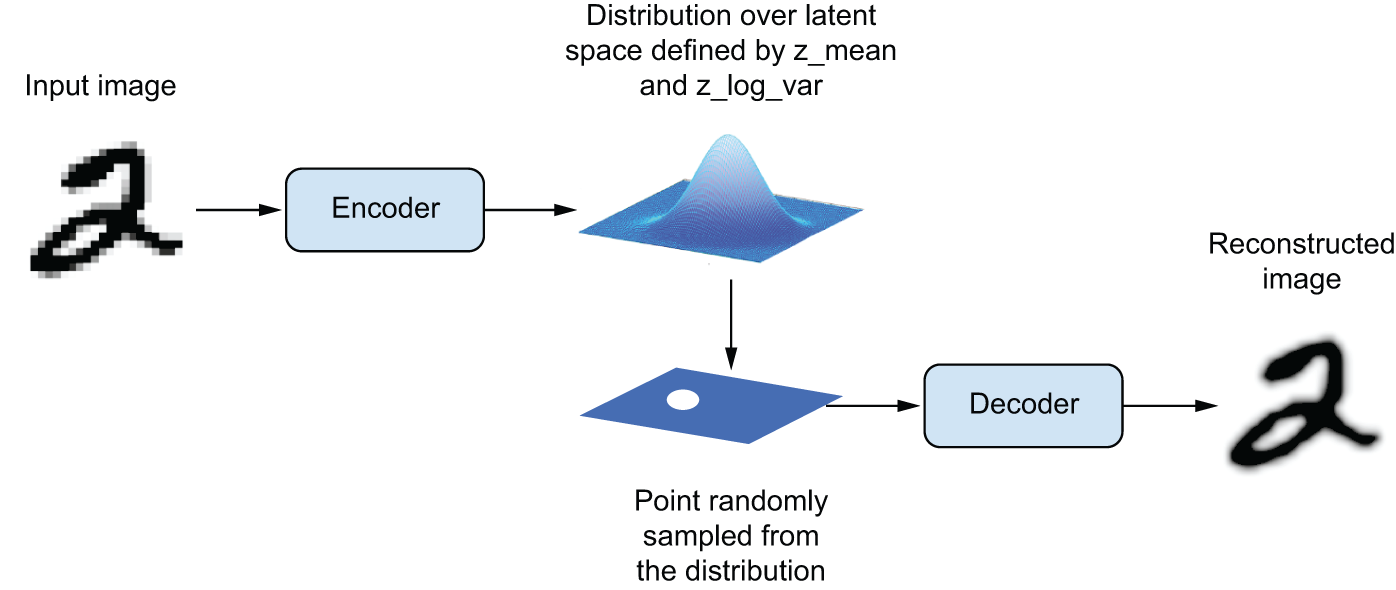
\includegraphics[width=\textwidth,height=0.6\textheight,keepaspectratio]{../../images/ch17/vae.df3af572.png}
            \caption{Cơ chế học Phân phối chuẩn của VAE}
        \end{figure}
    \end{columns}
\end{frame}

\begin{frame}[fragile]{Mã nguồn: Lớp Lấy mẫu (Sampler) của VAE}
\begin{lstlisting}[language=Python]
from keras import ops

class Sampler(keras.Layer):
    def __init__(self, **kwargs):
        super().__init__(**kwargs)
        # Seed generator for reproducible random sampling
        self.seed_generator = keras.random.SeedGenerator()
        self.built = True

    def call(self, z_mean, z_log_var):
        batch_size = ops.shape(z_mean)[0]
        z_size = ops.shape(z_mean)[1]
        epsilon = keras.random.normal(
            (batch_size, z_size), seed=self.seed_generator
        )
        # Applies the reparameterization trick
        return z_mean + ops.exp(0.5 * z_log_var) * epsilon
\end{lstlisting}
\end{frame}

\begin{frame}[fragile]{Mã nguồn: Mạng Bộ giải mã (Decoder) của VAE}
\begin{lstlisting}[language=Python]
import keras
from keras import layers

# Input where we'll feed z
latent_inputs = keras.Input(shape=(latent_dim,))
# Produces coefficients for reshaping
x = layers.Dense(7 * 7 * 64, activation="relu")(latent_inputs)
x = layers.Reshape((7, 7, 64))(x)
# Upsampling with Conv2DTranspose
x = layers.Conv2DTranspose(64, 3, activation="relu", strides=2, padding="same")(x)
x = layers.Conv2DTranspose(32, 3, activation="relu", strides=2, padding="same")(x)
# Final image output
decoder_outputs = layers.Conv2D(1, 3, activation="sigmoid", padding="same")(x)
decoder = keras.Model(latent_inputs, decoder_outputs, name="decoder")
\end{lstlisting}
\end{frame}

\begin{frame}{Toán học của VAE: Hàm mất mát KL Divergence}
    \begin{itemize}
        \item Hàm mất mát của VAE gồm 2 phần: Loss tái tạo (Reconstruction Loss) + KL Divergence Loss.
        \item \textbf{Kullback-Leibler (KL) Divergence:} Là thước đo Toán học ép Phân phối do Encoder sinh ra phải bám sát với Phân phối chuẩn $N(0, 1)$.
        \item Nhờ KL Loss, các điểm khái niệm không bị đẩy văng rải rác mà được gom tụ quy tâm, giúp việc di chuyển chuyển cảnh diễn ra mượt mà.
        \item Tuy nhiên, hàm mất mát tái tạo (dùng MSE/Binary Crossentropy) ép mô hình tính trung bình sai số điểm ảnh, dẫn đến ảnh sinh ra hay bị mờ (Blurry).
    \end{itemize}
\end{frame}

\begin{frame}[fragile]{Mã nguồn: Tính toán hàm mất mát cho VAE}
\begin{lstlisting}[language=Python]
class VAE(keras.Model):
    # compute_loss override to avoid specific backends logic
    def compute_loss(self, x, y, y_pred, sample_weight=None, training=True):
        z_mean, z_log_var = y_pred
        reconstruction = self.decoder(self.sampler(z_mean, z_log_var))

        # 1. Reconstruction Loss
        reconstruction_loss = ops.mean(
            ops.sum(keras.losses.binary_crossentropy(x, reconstruction), axis=(1, 2))
        )
        # 2. KL Divergence Loss
        kl_loss = -0.5 * (1 + z_log_var - ops.square(z_mean) - ops.exp(z_log_var))
        total_loss = reconstruction_loss + ops.mean(kl_loss)
        return total_loss
\end{lstlisting}
\end{frame}

\begin{frame}[fragile]{Mã nguồn: Lấy mẫu lưới điểm từ Không gian tiềm ẩn}
\begin{lstlisting}[language=Python]
import matplotlib.pyplot as plt
import numpy as np

# Samples points linearly on a 2D grid
grid_x = np.linspace(-1, 1, 30)
grid_y = np.linspace(-1, 1, 30)[::-1]

# Iterates over grid locations
for i, yi in enumerate(grid_y):
    for j, xi in enumerate(grid_x):
        # For each location, samples a digit and decodes it
        z_sample = np.array([[xi, yi]])
        x_decoded = vae.decoder.predict(z_sample)
        # Append decoded image to figure
        # ...
\end{lstlisting}
\end{frame}

\begin{frame}{Kết quả sinh ảnh từ VAE}
    \begin{columns}
        \column{0.5\textwidth}
        \begin{itemize}
            \item Không gian tiềm ẩn của VAE là một lưới liên tục.
            \item Khi ta di chuyển tuần tự qua các tọa độ của Không gian VAE, hình ảnh sẽ biến đổi (Morphing) trơn tru.
            \item Lưới các chữ số MNIST hiển thị sự phân bố liên tục: Các chữ số dần biến dạng từ 1 sang 7, từ 0 sang 9 theo phương hình học.
        \end{itemize}
        
        \column{0.5\textwidth}
        \begin{figure}
            \centering
            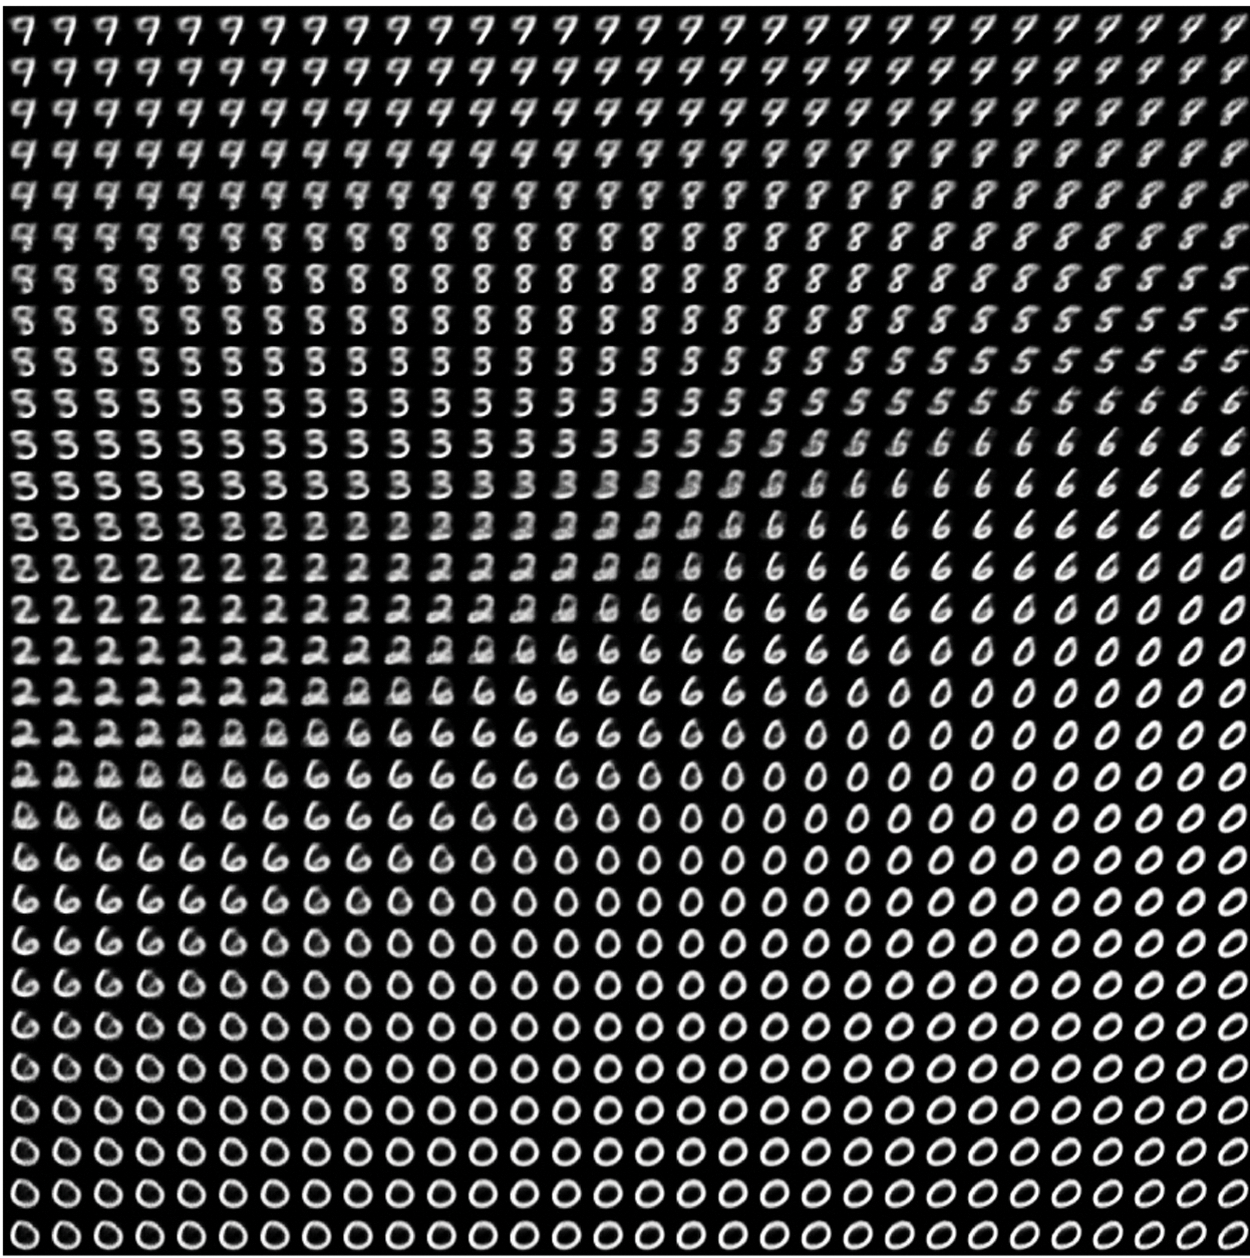
\includegraphics[width=\textwidth,height=0.6\textheight,keepaspectratio]{../../images/ch17/vae_grid.6152810c.png}
            \caption{Không gian nội suy ảnh chữ số MNIST của VAE}
        \end{figure}
    \end{columns}
\end{frame}

\section{3. Kỷ nguyên Diffusion Models}

\begin{frame}{Ứng dụng tiền thân: Nâng cao độ phân giải (Super Resolution)}
    \begin{columns}
        \column{0.5\textwidth}
        \begin{itemize}
            \item Trước khi Diffusion xuất hiện, mạng Autoencoder dùng để \textbf{Khử nhiễu (Denoising)}.
            \item Đưa một bức ảnh mờ nhiễu, mạng dự đoán và phục hồi bản gốc sắc nét.
            \item Nếu có thể khử nhiễu một chút, liệu ta có thể lặp lại vòng lặp khử nhiễu nhiều lần để biến một bức ảnh nhiễu hoàn toàn 100\% thành ảnh thật không?
        \end{itemize}
        
        \column{0.5\textwidth}
        \begin{figure}
            \centering
            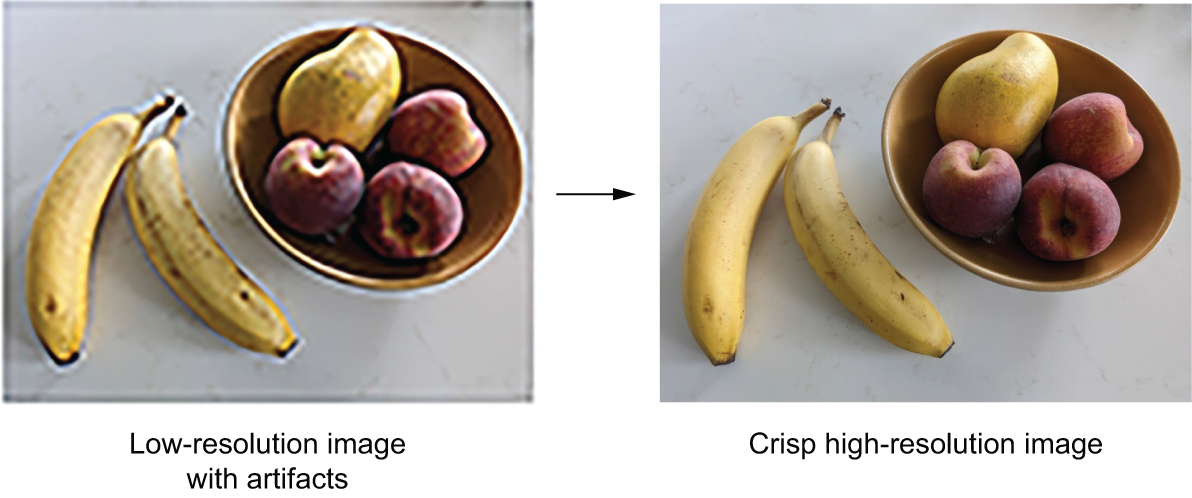
\includegraphics[width=\textwidth,height=0.6\textheight,keepaspectratio]{../../images/ch17/superresolution.0d8b50ab.png}
            \caption{Phục hồi ảnh bằng Siêu phân giải}
        \end{figure}
    \end{columns}
\end{frame}

\begin{frame}{Mô hình Khuếch tán (Diffusion Models)}
    \begin{columns}
        \column{0.5\textwidth}
        \begin{itemize}
            \item \textbf{Forward Diffusion:} Phá hủy ảnh gốc bằng cách thêm nhiễu (Noise) ngẫu nhiên dần dần cho đến khi chỉ còn tĩnh nhiễu trắng (Pure noise).
            \item \textbf{Reverse Diffusion (Backward):} Huấn luyện mạng Nơ-ron (U-Net) học cách gỡ bỏ nhiễu từng bước một để khôi phục ảnh từ hư vô.
            \item Tương tự như việc điêu khắc một bức tượng từ một khối đá vô định.
        \end{itemize}
        
        \column{0.5\textwidth}
        \begin{figure}
            \centering
            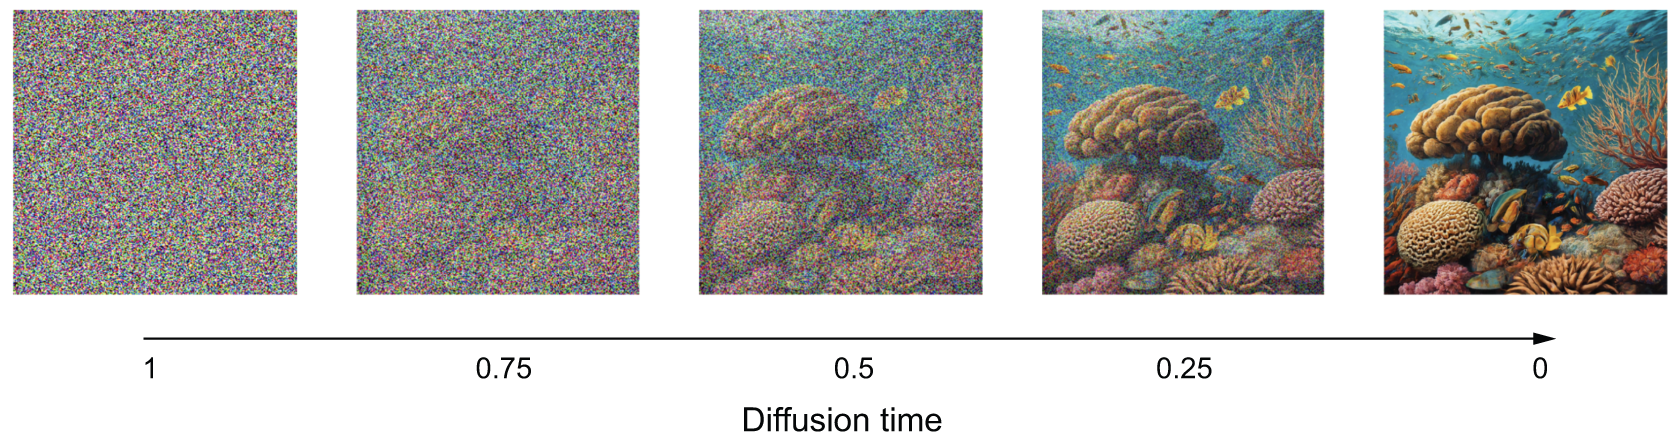
\includegraphics[width=\textwidth,height=0.6\textheight,keepaspectratio]{../../images/ch17/diffusion.184e1d12.png}
            \caption{Tiến trình Forward và Backward của Diffusion}
        \end{figure}
    \end{columns}
\end{frame}

\begin{frame}{Lịch trình thêm nhiễu (Noise Schedule)}
    \begin{columns}
        \column{0.5\textwidth}
        \begin{itemize}
            \item Lượng nhiễu thêm vào ở mỗi bước thời gian $t$ không được ngẫu nhiên mà tuân theo một \textbf{Noise Schedule} (Linear, Cosine,...).
            \item \textbf{Cosine Schedule:} Đảm bảo sự cân bằng mượt mà giữa Tỷ lệ Tín hiệu (Signal rate) và Tỷ lệ Nhiễu (Noise rate) theo hệ thức $\text{noise}^2 + \text{signal}^2 = 1$.
        \end{itemize}
        
        \column{0.5\textwidth}
        \begin{figure}
            \centering
            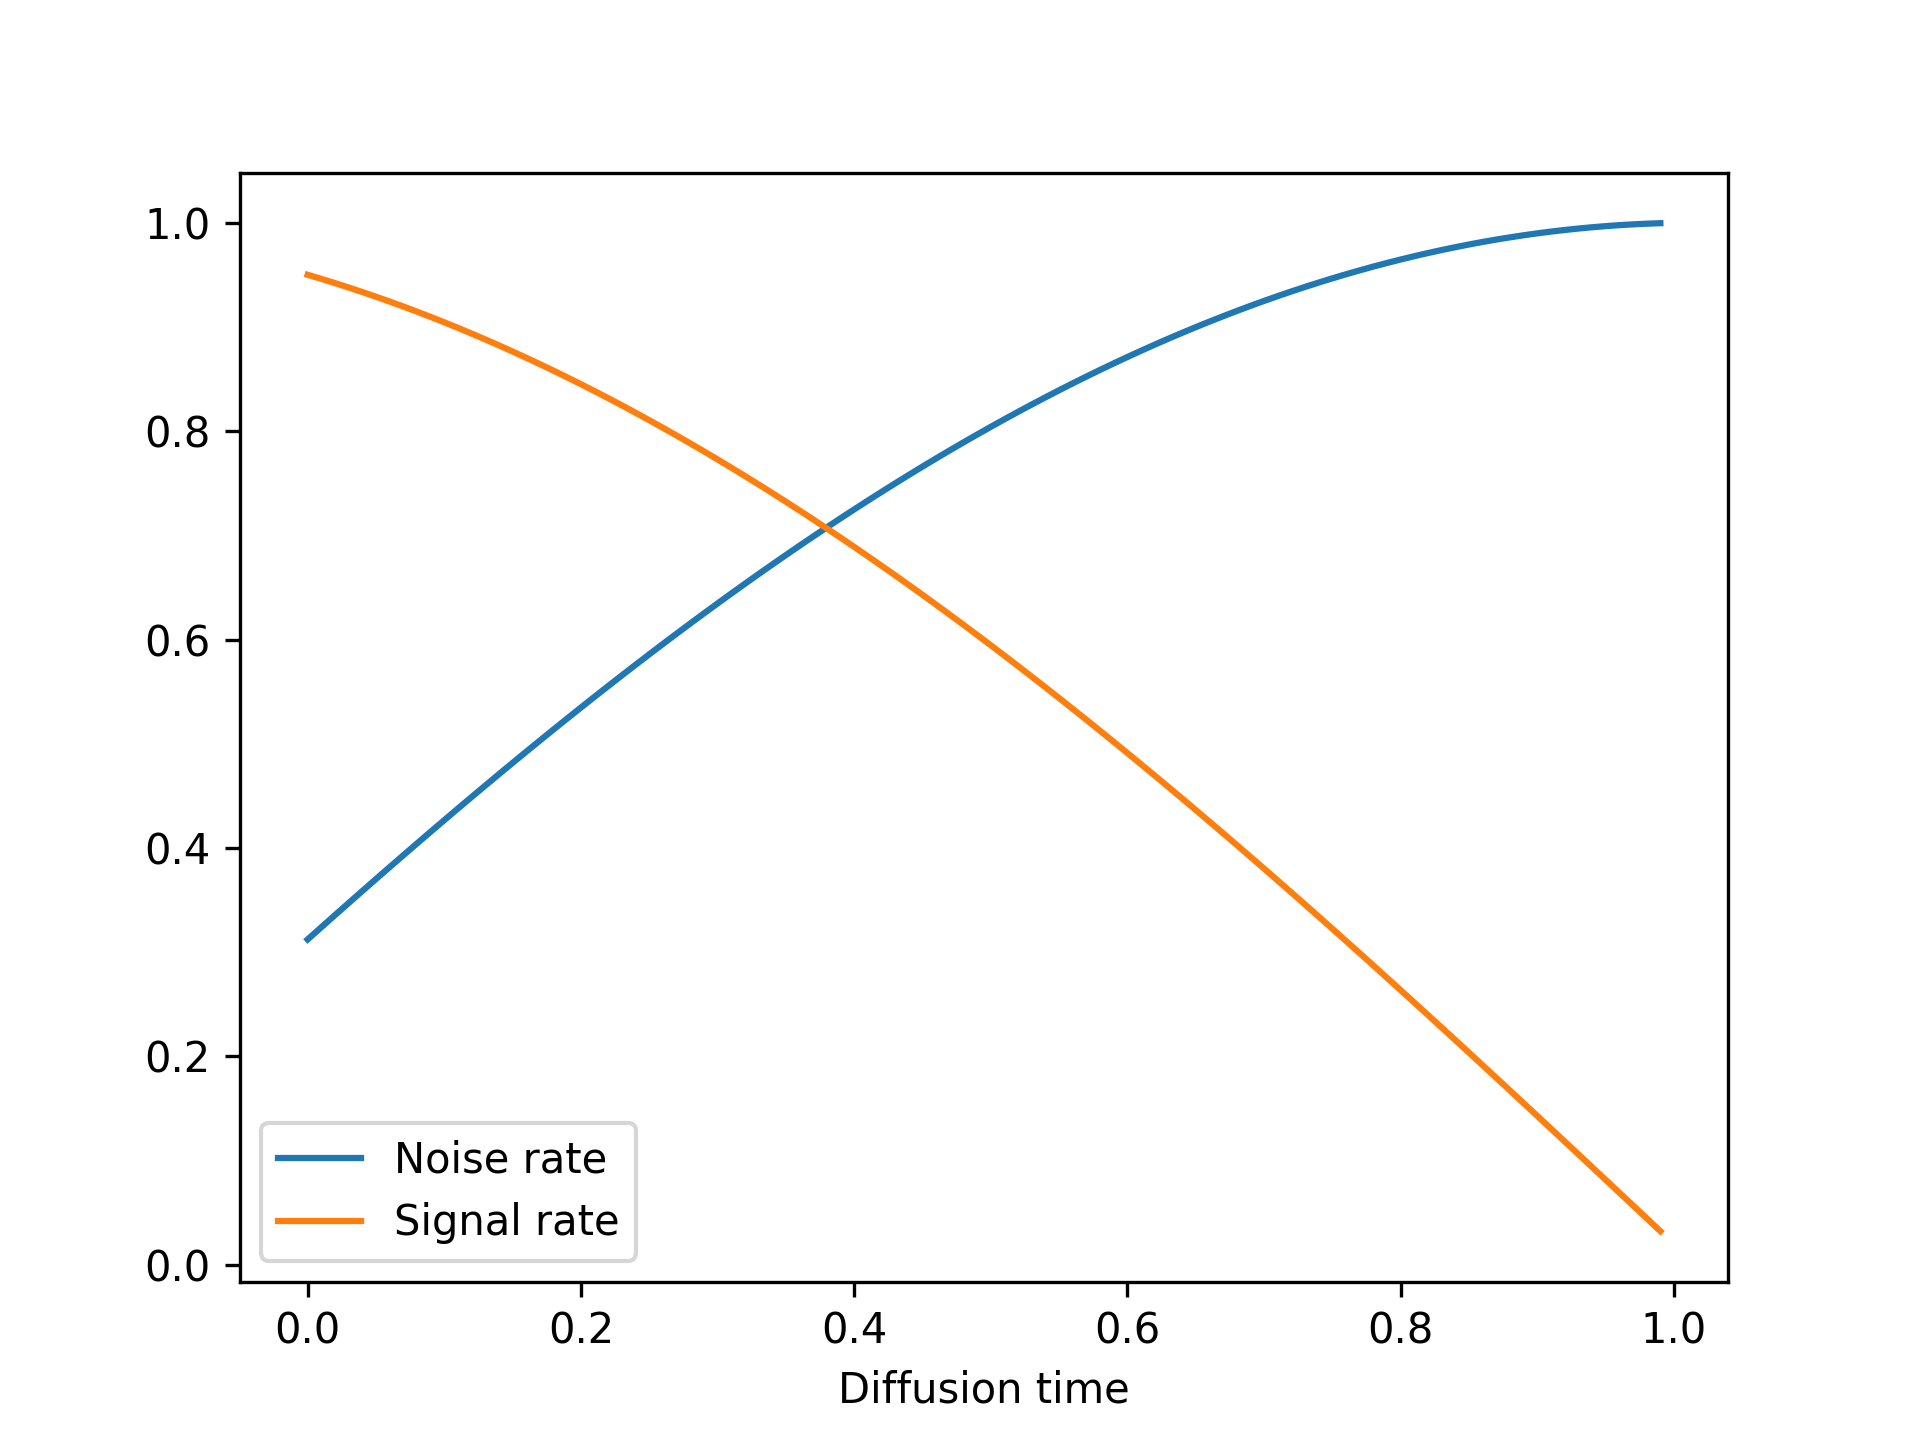
\includegraphics[width=\textwidth,height=0.6\textheight,keepaspectratio]{../../images/ch17/diffusion_schedule.52ecea17.png}
            \caption{Đồ thị Lịch trình Nhạy nhiễu Cosine}
        \end{figure}
    \end{columns}
\end{frame}

\begin{frame}{Góc độ Hình học của Cosine trong Diffusion}
    \begin{columns}
        \column{0.5\textwidth}
        \begin{itemize}
            \item Việc tính toán tỷ lệ tín hiệu và nhiễu dựa trên góc độ pha $\Omega$ thay đổi từ $0$ đến $\frac{\pi}{2}$.
            \item Hàm cosine và sine được sử dụng làm trọng số nội suy.
            \item Giúp duy trì cường độ không gian (Variance) của dữ liệu ở mọi bước (luôn ổn định bằng 1), chống suy giảm tính ổn định số học.
        \end{itemize}
        
        \column{0.5\textwidth}
        \begin{figure}
            \centering
            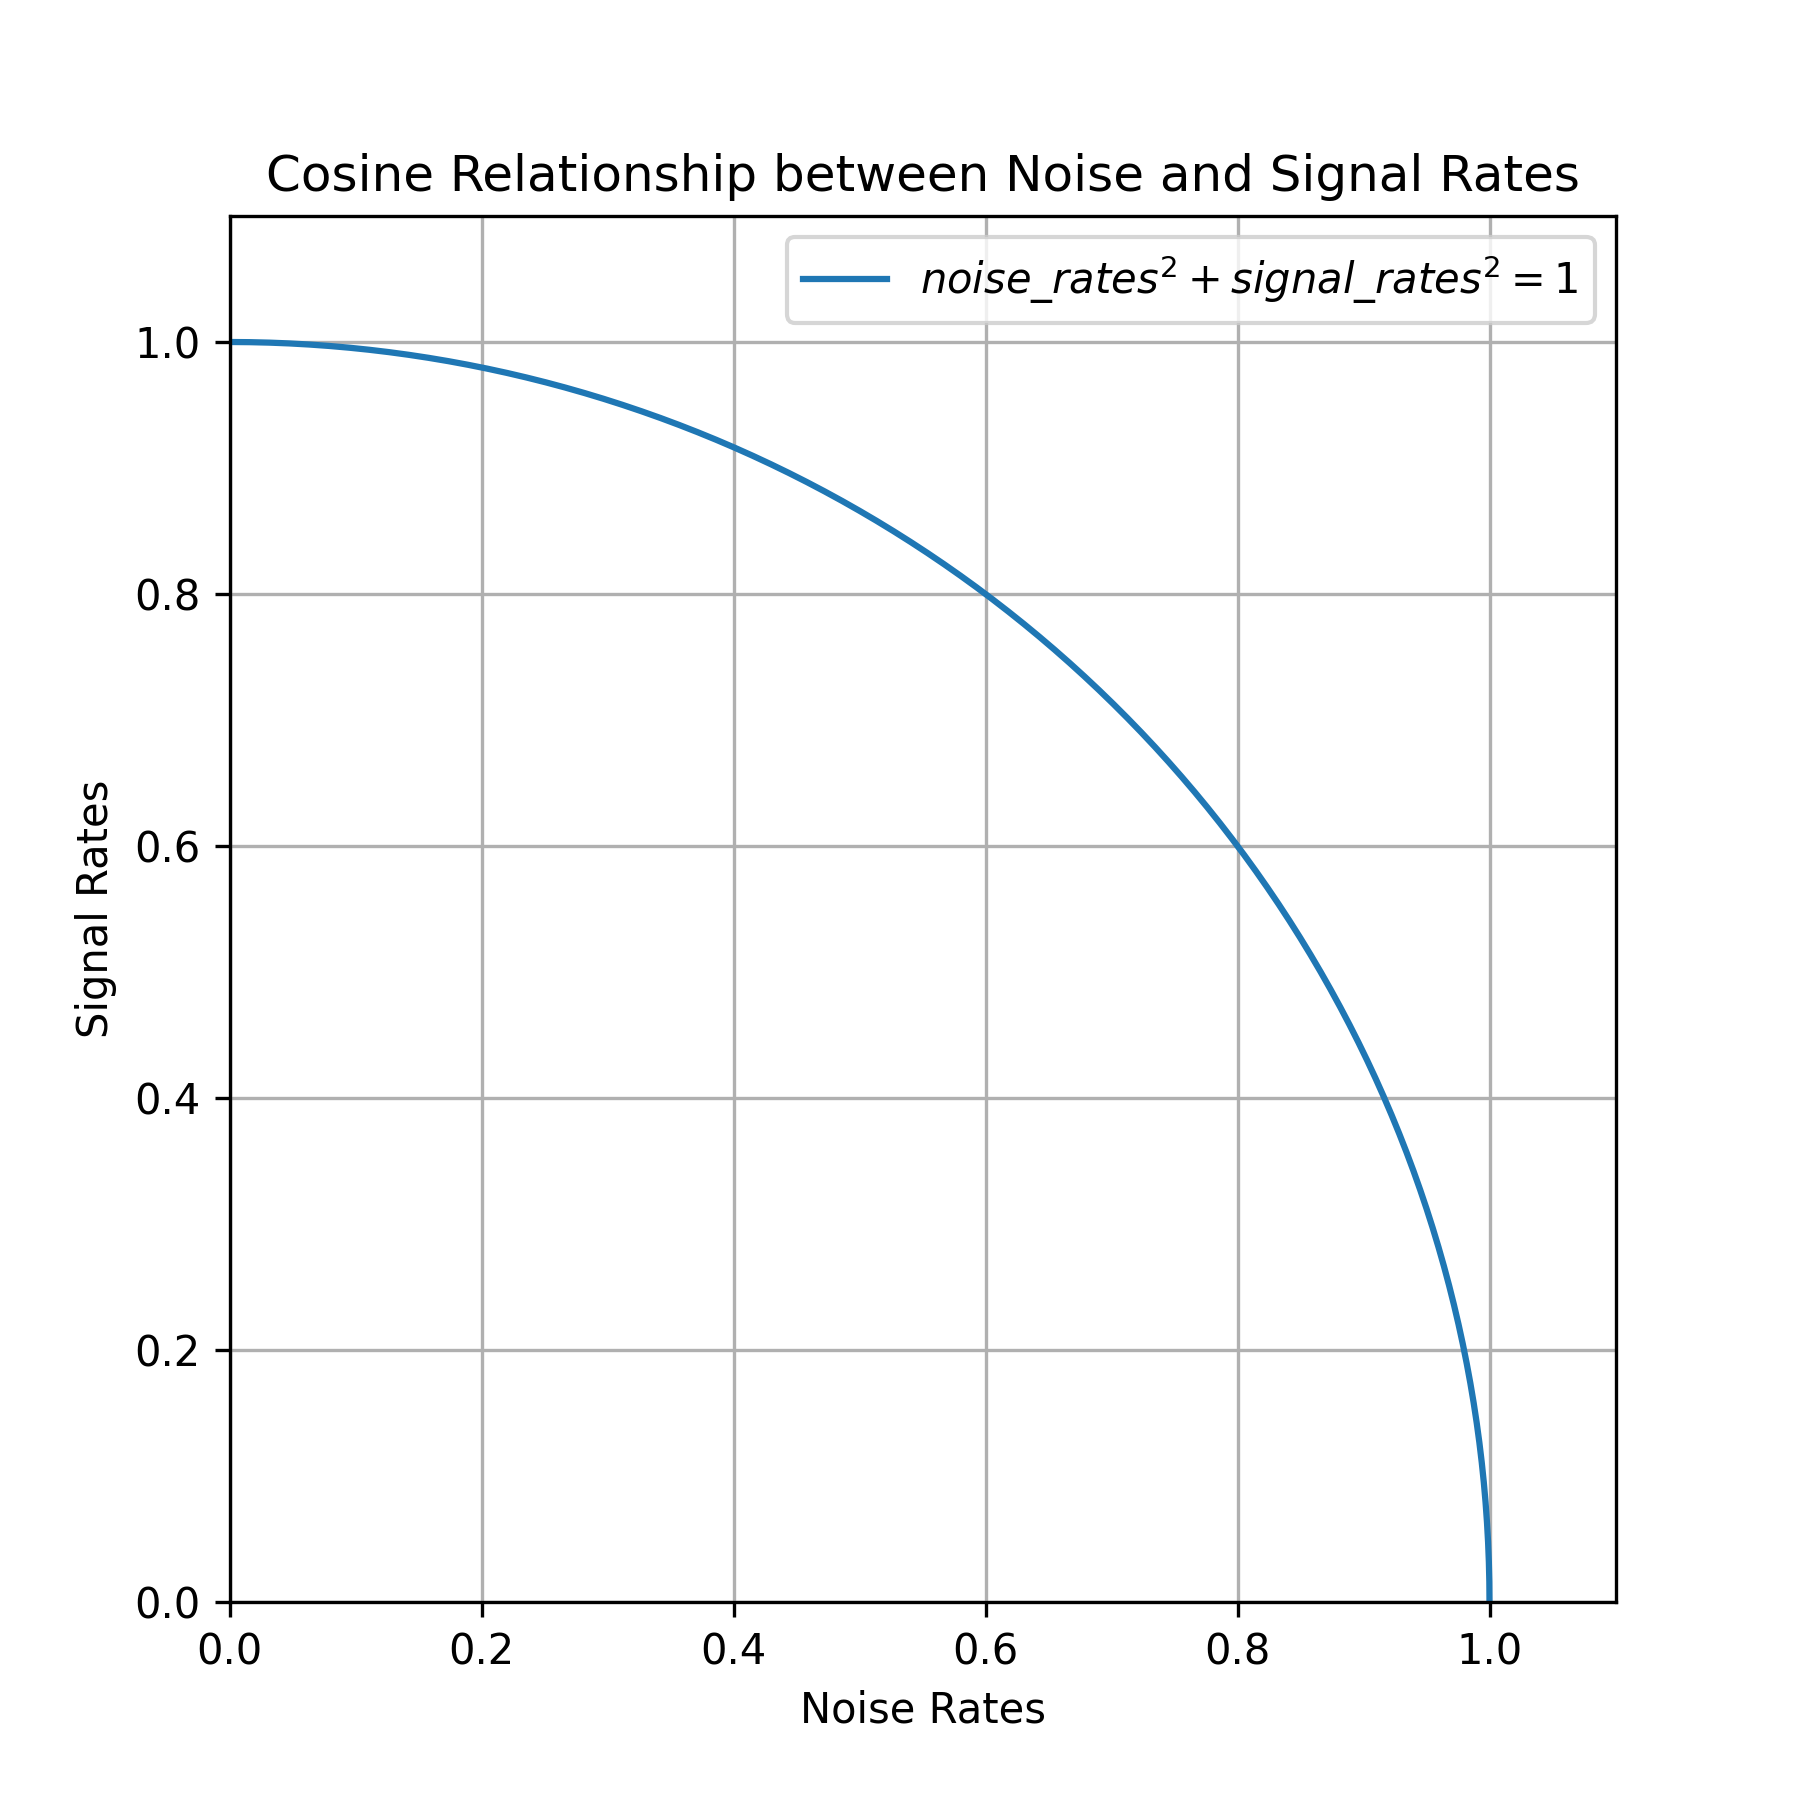
\includegraphics[width=\textwidth,height=0.6\textheight,keepaspectratio]{../../images/ch17/cosine_relationship.c5f419f0.png}
            \caption{Mối quan hệ hình học Cosine giữa Tín hiệu và Nhiễu}
        \end{figure}
    \end{columns}
\end{frame}

\begin{frame}{Mạng U-Net khử nhiễu}
    \begin{columns}
        \column{0.5\textwidth}
        \begin{itemize}
            \item Trái tim của Diffusion chính là \textbf{Mạng U-Net}.
            \item \textbf{Cấu trúc 3 giai đoạn:} Downsampling (giảm lấy mẫu nén đặc trưng), Middle stage (khối trung tâm), Upsampling (tăng lấy mẫu phục hồi độ phân giải).
            \item \textbf{Skip-Connections (Kết nối dư):} Nối liền các lớp từ Downsampling sang Upsampling giúp mô hình không bị mất các chi tiết ảnh sắc nét vi mô.
        \end{itemize}
        
        \column{0.5\textwidth}
        \begin{figure}
            \centering
            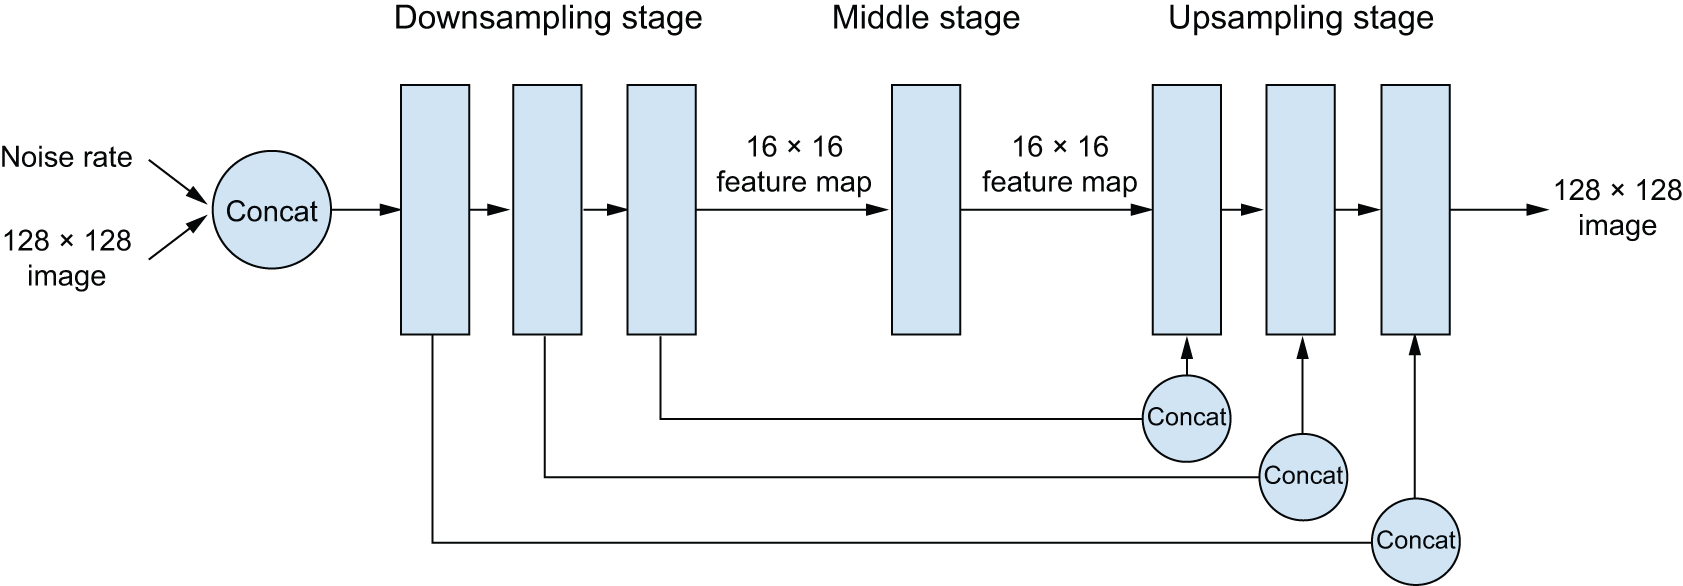
\includegraphics[width=\textwidth,height=0.6\textheight,keepaspectratio]{../../images/ch17/unet.20eacd7d.png}
            \caption{Sơ đồ kiến trúc U-Net kinh điển với Skip Connections}
        \end{figure}
    \end{columns}
\end{frame}

\begin{frame}[fragile]{Mã nguồn: Lịch trình Khuếch tán Cosine}
\begin{lstlisting}[language=Python]
def diffusion_schedule(
    diffusion_times, min_signal_rate=0.02, max_signal_rate=0.95,
):
    # Calculate angles for cosine schedule
    start_angle = ops.cast(ops.arccos(max_signal_rate), "float32")
    end_angle = ops.cast(ops.arccos(min_signal_rate), "float32")
    diffusion_angles = start_angle + diffusion_times * (end_angle - start_angle)
    
    # Calculate signal and noise rates maintaining square sum = 1
    signal_rates = ops.cos(diffusion_angles)
    noise_rates = ops.sin(diffusion_angles)
    return noise_rates, signal_rates
\end{lstlisting}
\end{frame}

\begin{frame}[fragile]{Mã nguồn: Tính toán Bước khử nhiễu (Denoise)}
\begin{lstlisting}[language=Python]
class DiffusionModel(keras.Model):
    # ...
    def denoise(self, noisy_images, noise_rates, signal_rates):
        # Calls the denoising UNet model
        pred_noise_masks = self.denoising_model([noisy_images, noise_rates])
        # Reconstructs the predicted clean image using algebraic rearrangement
        pred_images = (
            noisy_images - noise_rates * pred_noise_masks
        ) / signal_rates
        return pred_images, pred_noise_masks
\end{lstlisting}
\end{frame}

\begin{frame}[fragile]{Mã nguồn: Tiến trình Sinh ảnh ngẫu nhiên (Generation)}
\begin{lstlisting}[language=Python]
def generate(self, num_images, diffusion_steps):
    # Starts from pure noise
    noisy_images = keras.random.normal(
        (num_images, self.image_size, self.image_size, 3), seed=self.seed_generator
    )
    step_size = 1.0 / diffusion_steps
    for step in range(diffusion_steps):
        # Loop to progressively remove noise
        diffusion_times = ops.ones((num_images, 1, 1, 1)) - step * step_size
        noise_rates, signal_rates = diffusion_schedule(diffusion_times)
        pred_images, pred_noises = self.denoise(noisy_images, noise_rates, signal_rates)
        # Prepares noisy images for the next iteration
        next_diffusion_times = diffusion_times - step_size
        next_noise_rates, next_signal_rates = diffusion_schedule(next_diffusion_times)
        noisy_images = next_signal_rates * pred_images + next_noise_rates * pred_noises
    # Denormalize to 0-255 pixels
    # ...
\end{lstlisting}
\end{frame}

\begin{frame}[fragile]{Mã nguồn: Kỹ thuật ổn định huấn luyện Diffusion}
\begin{lstlisting}[language=Python]
model.compile(
    optimizer=keras.optimizers.AdamW(
        # Configures the learning rate decay schedule
        learning_rate=keras.optimizers.schedules.InverseTimeDecay(
            initial_learning_rate=1e-3, decay_steps=1000, decay_rate=0.1,
        ),
        # Turns on Polyak averaging (Exponential Moving Average)
        use_ema=True,
        # Overwrite the weights with EMA every 100 iterations
        ema_overwrite_frequency=100,
    ),
)
\end{lstlisting}
\end{frame}

\begin{frame}{Ý nghĩa của Kỹ thuật Polyak Averaging (EMA)}
    \begin{itemize}
        \item Mô hình Diffusion rất khó hội tụ và có nhiều đỉnh nhiễu loạn trong Không gian mất mát (Loss Landscape).
        \item Nếu chỉ lưu trọng số sau mỗi Epoch bình thường, mô hình có thể bị vướng vào cục bộ nhiễu.
        \item \textbf{Polyak Averaging (EMA):} Lưu trữ trung bình cộng theo cấp số nhân của các trọng số quá khứ. Cứ 100 bước ta ghi đè bằng trọng số trung bình này, giúp đường đi huấn luyện ổn định mượt mà hơn rất nhiều.
    \end{itemize}
\end{frame}

\begin{frame}{Kết quả sinh ảnh hoa từ Diffusion}
    \begin{columns}
        \column{0.5\textwidth}
        \begin{itemize}
            \item Trái ngược với VAE, Diffusion cần thực hiện lặp lại U-Net rất nhiều lần (Sampling steps), nên tốc độ chậm hơn đáng kể.
            \item \textbf{Đổi lại:} Chất lượng hình ảnh cực kỳ sắc nét, sinh động, sửa chữa hoàn toàn yếu điểm hình ảnh bị mờ đục của VAE và GAN.
            \item Đây là xương sống cho mọi hệ thống Sinh ảnh hiện đại.
        \end{itemize}
        
        \column{0.5\textwidth}
        \begin{figure}
            \centering
            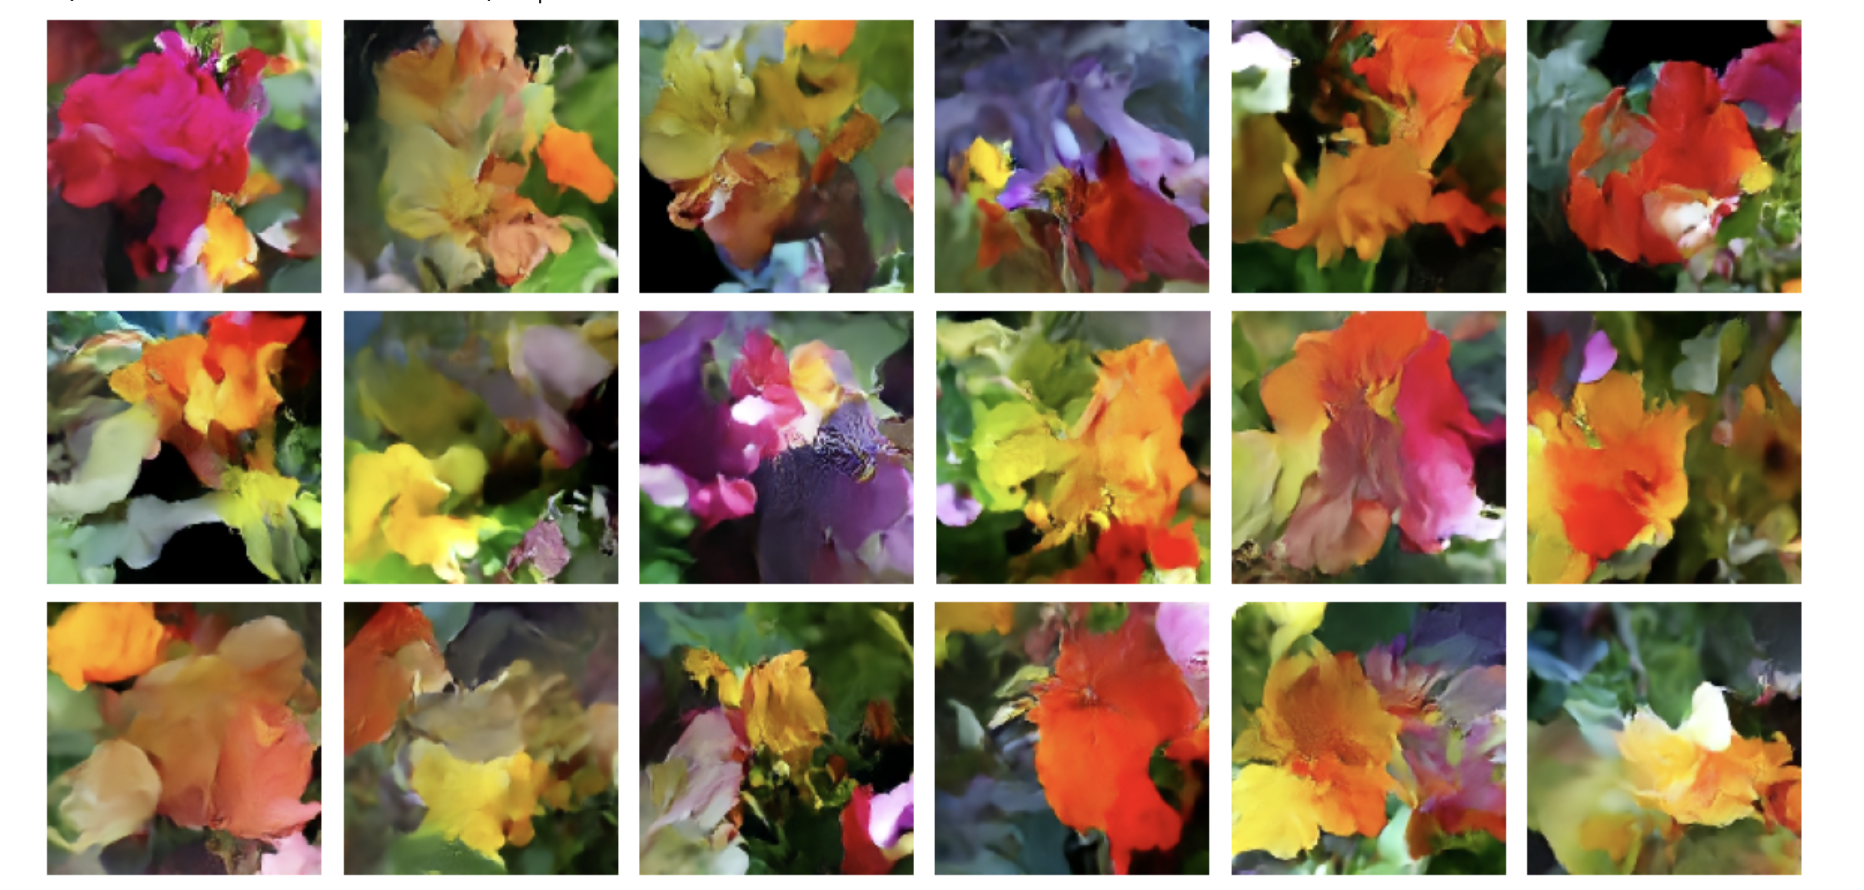
\includegraphics[width=\textwidth,height=0.6\textheight,keepaspectratio]{../../images/ch17/generated_flowers.614c95f0.png}
            \caption{Hình ảnh hoa sắc nét sinh từ Diffusion}
        \end{figure}
    \end{columns}
\end{frame}

\section{4. Stable Diffusion \& Kỹ thuật nâng cao}

\begin{frame}{Nhược điểm của Standard Diffusion và Sự ra đời của Stable Diffusion}
    \begin{itemize}
        \item Thực thi Diffusion trực tiếp trên Không gian Pixel khổng lồ (Ví dụ ảnh $1024 \times 1024$) tốn kém thời gian nội suy và VRAM.
        \item \textbf{Stable Diffusion (Latent Diffusion Model):} Bức phá bằng cách kết hợp sức mạnh VAE và Diffusion.
        \item Chạy tiến trình Thêm nhiễu và Khử nhiễu trên \textbf{Không gian tiềm ẩn (Latent space) nén nhỏ của VAE} (Ví dụ lưới vector $64 \times 64$). 
        \item Giúp SD chạy mượt mà ngay trên PC hoặc Laptop chỉ trong vài giây.
    \end{itemize}
\end{frame}

\begin{frame}{Kết quả từ Stable Diffusion 3}
    \begin{columns}
        \column{0.5\textwidth}
        \begin{itemize}
            \item Stable Diffusion dùng Bộ mã hóa văn bản (Text Encoder) để nhúng Prompt thành Context nuôi mạng U-Net.
            \item Có khả năng tạo ra hình ảnh phi thực tế theo Lời nhắc: \textit{"A NASA astronaut riding an origami elephant in New York City"}.
            \item Hoạt động linh hoạt chỉ với thư viện mã nguồn mở KerasHub API.
        \end{itemize}
        
        \column{0.5\textwidth}
        \begin{figure}
            \centering
            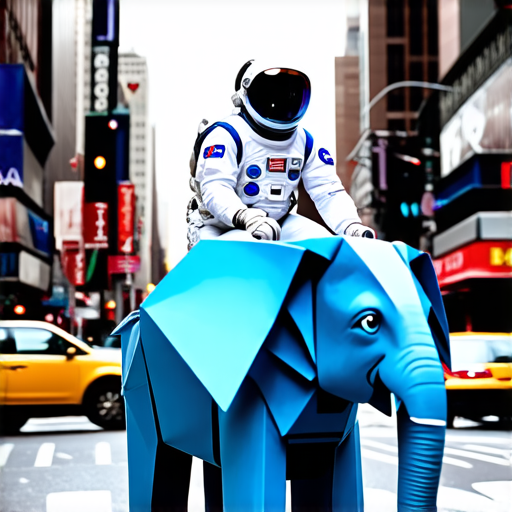
\includegraphics[width=\textwidth,height=0.6\textheight,keepaspectratio]{../../images/ch17/sd3-output.6c189acc.png}
            \caption{Bức ảnh phi hành gia sinh ra từ Stable Diffusion 3}
        \end{figure}
    \end{columns}
\end{frame}

\begin{frame}{Tác động của Số bước Khử nhiễu (Denoising Steps)}
    \begin{columns}
        \column{0.5\textwidth}
        \begin{itemize}
            \item Quá trình sinh ảnh chạy bằng vòng lặp $N$ bước.
            \item Nếu $N$ quá nhỏ (VD: 5 bước), thuật toán giải mã chưa hội tụ, ảnh đọng lại hạt nhiễu xám (Noise artifacts).
            \item Tăng $N$ (20 - 50 bước) giúp hình hoàn thiện sắc nét. Số bước lớn hơn không tăng thêm chi tiết mà gây lãng phí bộ đếm thời gian.
        \end{itemize}
        
        \column{0.5\textwidth}
        \begin{figure}
            \centering
            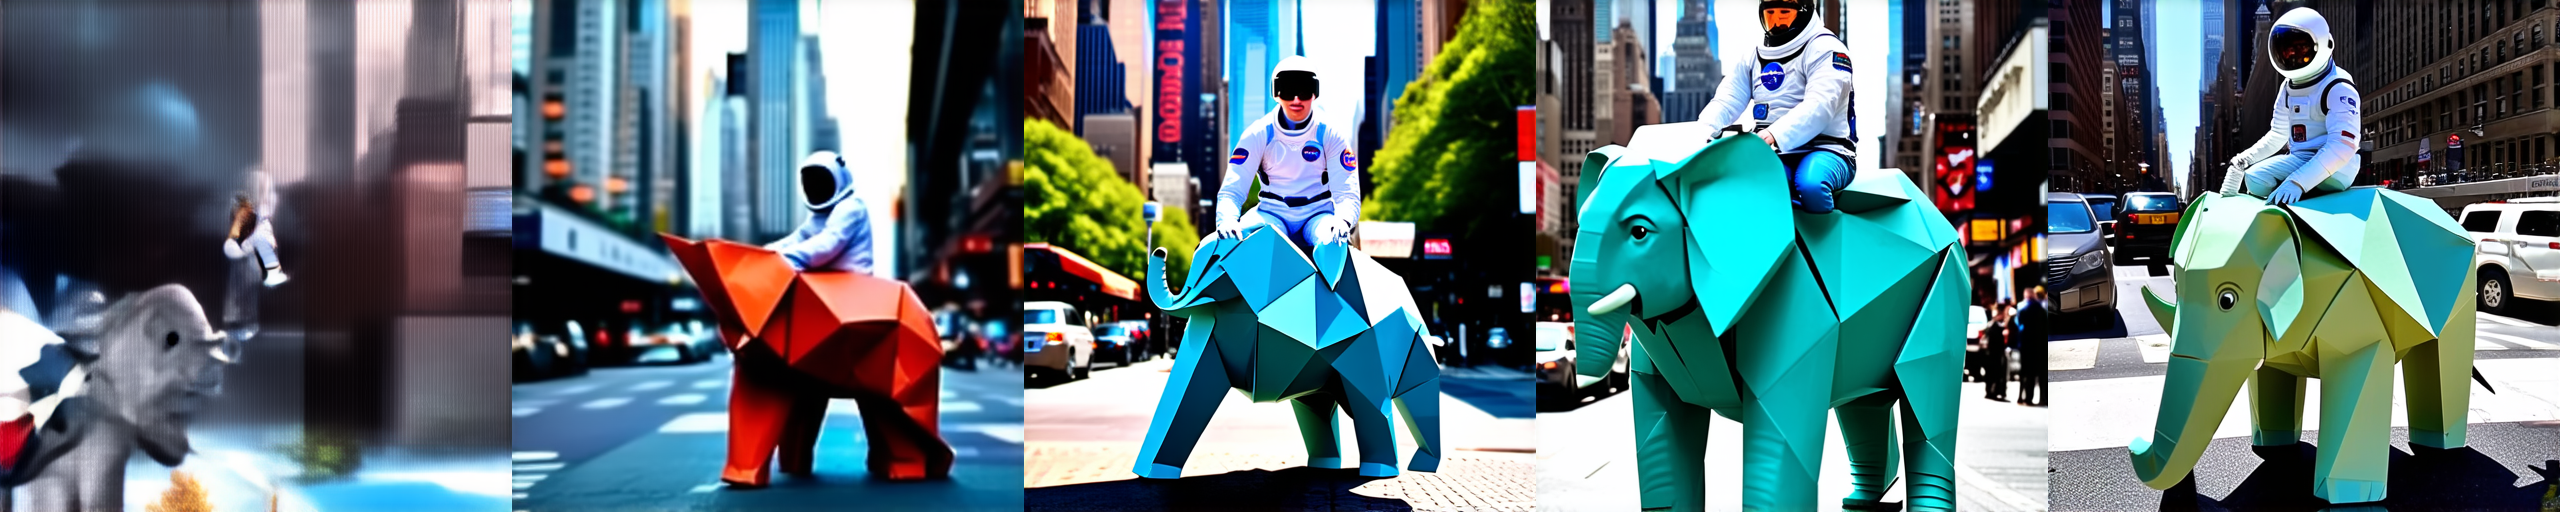
\includegraphics[width=\textwidth,height=0.6\textheight,keepaspectratio]{../../images/ch17/sd3-output-steps.c490d938.png}
            \caption{Sự thay đổi độ chi tiết ảnh theo số bước Denoise}
        \end{figure}
    \end{columns}
\end{frame}

\begin{frame}{Sức mạnh của Negative Prompt (Lời nhắc tiêu cực)}
    \begin{columns}
        \column{0.5\textwidth}
        \begin{itemize}
            \item Khi mô hình sinh chi tiết lỗi (màu sắc không chuẩn, mờ, thiếu ngón, biến dạng).
            \item \textbf{Negative Prompt:} Hoạt động dựa trên Classifier-Free Guidance (CFG). Hệ thống trích xuất vector Tích cực và Tiêu cực, sau đó ép bước lặp \textbf{di chuyển ngược chiều hướng Tiêu cực}.
        \end{itemize}
        
        \column{0.5\textwidth}
        \begin{figure}
            \centering
            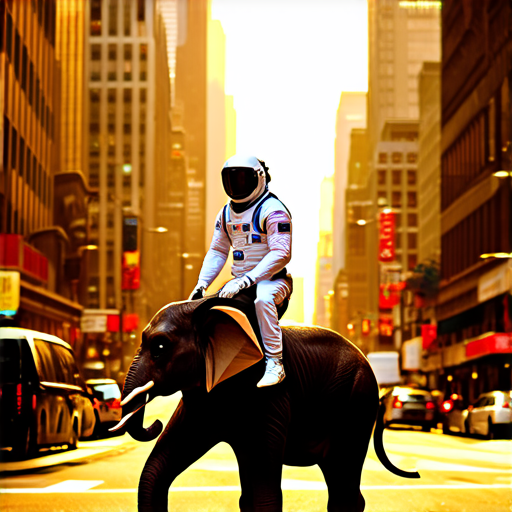
\includegraphics[width=\textwidth,height=0.6\textheight,keepaspectratio]{../../images/ch17/sd3-output-negative.32fbdbe2.png}
            \caption{Loại bỏ màu xanh (Blue color) bằng Negative Prompt}
        \end{figure}
    \end{columns}
\end{frame}

\begin{frame}{Nội suy hình học trong Không gian tiềm ẩn}
    \begin{columns}
        \column{0.5\textwidth}
        \begin{itemize}
            \item Không gian tiềm ẩn của Diffusion rất liên kết và mịn màng.
            \item Lấy điểm $A$ và $B$, tính toán các tọa độ nằm giữa 2 vector. Giải mã chúng giúp tạo ra hiệu ứng \textbf{Morphing} (Biến hình) trơn tru chuyển cảnh.
            \item Đây là bước đệm phát triển thuật toán Text-to-Video đỉnh cao hiện hành.
        \end{itemize}
        
        \column{0.5\textwidth}
        \begin{figure}
            \centering
            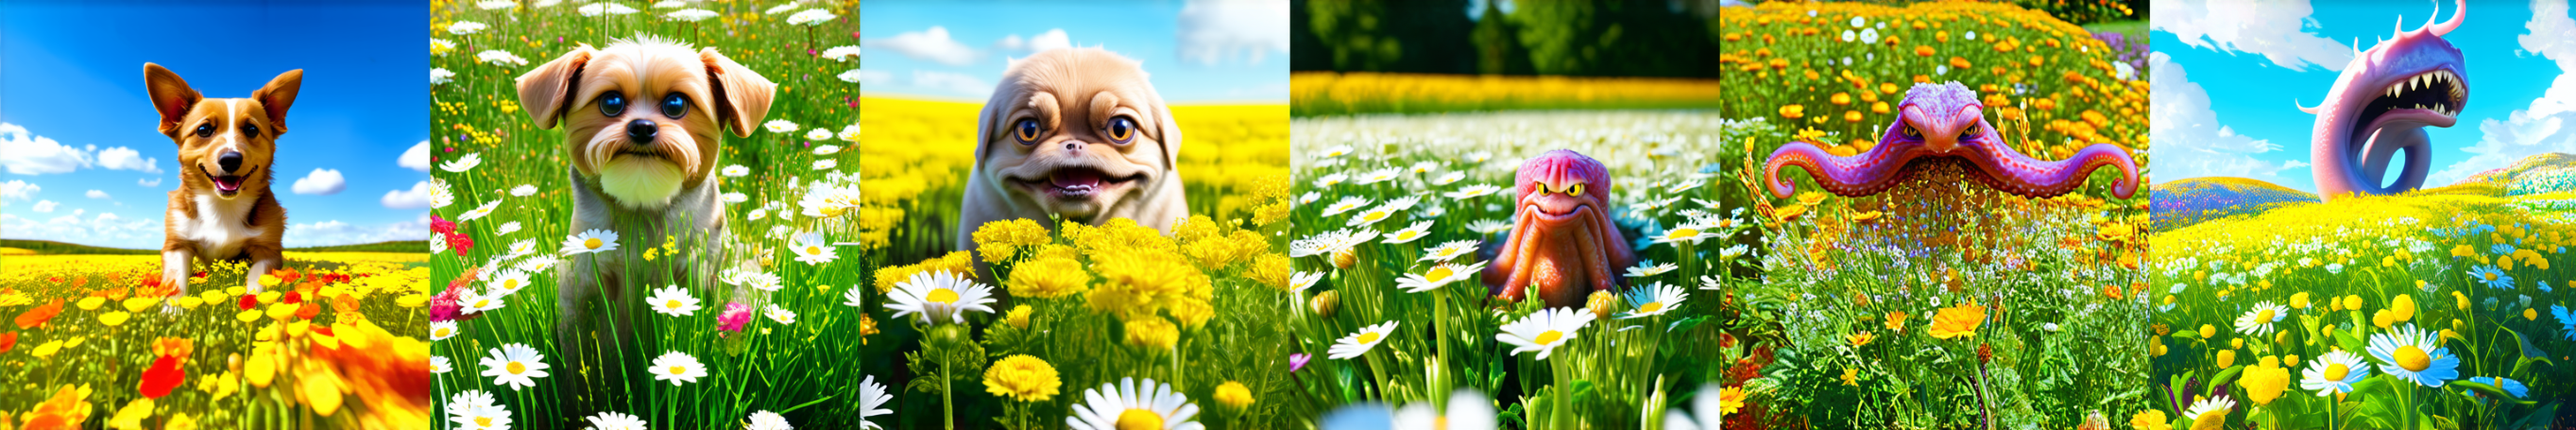
\includegraphics[width=\textwidth,height=0.6\textheight,keepaspectratio]{../../images/ch17/sd3-morph.40f60bd8.png}
            \caption{Hiệu ứng chuyển cảnh trong Latent Space}
        \end{figure}
    \end{columns}
\end{frame}

\begin{frame}{Toán học Nội suy cầu (SLERP)}
    \begin{columns}
        \column{0.5\textwidth}
        \begin{itemize}
            \item Trong không gian nhiều chiều ($D \approx 4096$), nội suy tuyến tính (Linear) làm đường thẳng cắt ngang tâm cầu, gây vỡ ảnh khúc giữa.
            \item \textbf{Giải pháp: Spherical Linear Interpolation (SLERP)}. Tính góc Cosine $\Omega$, giữ hướng đi bám cung tròn bề mặt không gian sinh thái.
            $$ SLERP = \frac{\sin((1-t)\Omega)}{\sin(\Omega)}p_0 + \frac{\sin(t\Omega)}{\sin(\Omega)}p_1 $$
        \end{itemize}
        
        \column{0.5\textwidth}
        \begin{figure}
            \centering
            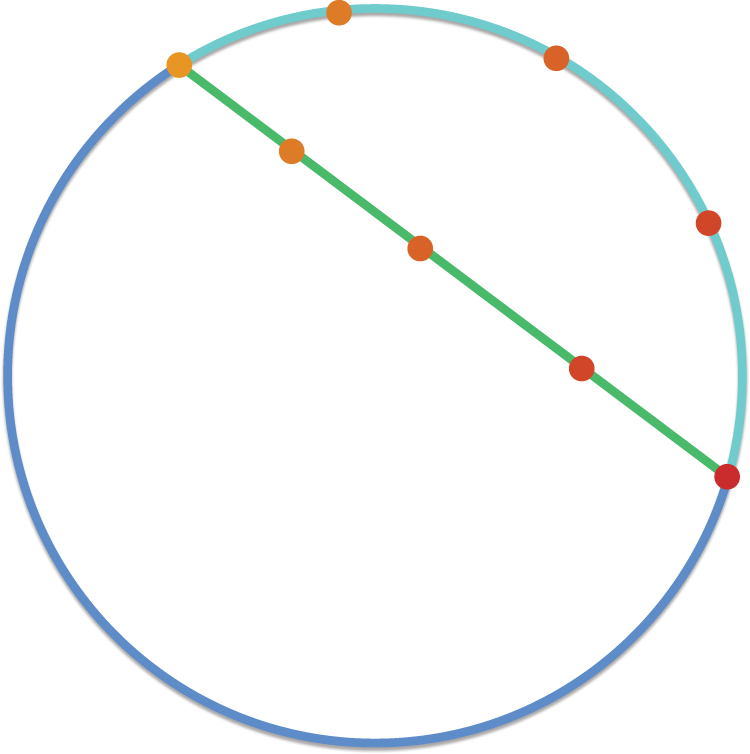
\includegraphics[width=\textwidth,height=0.6\textheight,keepaspectratio]{../../images/ch17/slerp.eea42213.png}
            \caption{Minh họa đường đi SLERP cong bám trên cung cầu}
        \end{figure}
    \end{columns}
\end{frame}

\section{Tổng kết}

\begin{frame}{Tổng kết Chương 17}
    \begin{itemize}
        \item \textbf{VAE:} Tiên phong với Không gian tiềm ẩn liên tục học qua phương sai và KL Divergence. Chất lượng hình ảnh kém sắc nét do MSE Loss.
        \item \textbf{Diffusion Models:} Lật đổ VAE nhờ tiến trình Thêm nhiễu và Khử nhiễu qua mạng U-Net, trả về bức ảnh nét đến từng điểm ảnh.
        \item \textbf{Kỹ thuật huấn luyện tối ưu:} Sử dụng Polyak Averaging (EMA) chống kẹt cực tiểu địa phương trong lúc huấn luyện Gradient.
        \item \textbf{Stable Diffusion:} Nén quá trình Denoise vào Latent Space, tích hợp Prompt/Negative Prompts, thay đổi hoàn toàn cách sinh ảnh dân dụng.
        \item \textbf{Toán học không gian:} Áp dụng SLERP di chuyển mượt mà trên không gian biểu diễn đa chiều cho Morphing Video.
    \end{itemize}
\end{frame}

\end{document}
